\chapter{Vers des fonctions de qualité dans les flots de liens}
\minitoc
\label{versQualite}

Nous avons vu dans le chapitre précédent que la génération d'exemples ayant une structure connue est un atout pour tester et valider des fonctions de qualité.
Pour être utile à la validation de fonction de qualité, un générateur doit être capable de construire des systèmes ayant des caractéristiques vraisemblables de structures communautaires.
Pour ce faire, plusieurs contraintes peuvent être considérées selon le degré de liberté du système généré.
Dans le cas des graphes, le premier générateur est celui de Erdös-Rényi qui fixe le nombre de liens et ainsi la densité mais où il n'y existe \emph{a priori} pas de structure.
D'autres générateurs ont été proposés pour intégrer une structure comme \emph{planted partition} ou LFR.
Ce domaine de recherche est d'ailleurs toujours vivant~\cite{Tabourier2011,Obradovic2014} car il est parfois nécessaire d'intégrer de nouvelles contraintes sur le graphe généré.
Il existe cependant peu de méthode pour générer des réseaux dynamiques que ce soit sous la forme de série de graphes, de graphes temporel ou de flots de liens.


Dans ce chapitre, nous présentons un premier générateur de flots de liens sans durée avec une structure communautaire sur les liens.
L'intuition derrière ce générateur est la suivante.
L'apparition des liens entre deux n\oe uds dépendent uniquement des communautés que partagent ces deux n\oe uds.
Si ils n'ont aucune communauté en commun alors il n'y aura pas ou peu de liens entre ces n\oe uds.
Plus ils partagent de communautés, plus il y existera de liens entre ces n\oe uds.
De plus comme un lien est généré à cause d'une communauté partagée par deux n\oe uds, il est possible d'assigner à ce lien la communauté partagée par ces n\oe uds.
Grâce à ce générateur, il est possible de générer différents flots de liens et de tester des fonctions de qualité et des méthodes de détections.

Nous tirons partis de ce générateur de deux façon différentes sur des pistes qui sont encore exploratoires.
Tout d'abord, nous testons différentes méthodes de détections de communautés statique sur des projections du flot de liens.
Puis, nous proposons et étudions différentes fonctions de qualité dans une approche similaire à \emph{Expeted Nodes}.

\bigskip

Le chapitre est organisé de la manière suivante.
Dans la section~\ref{sec:versqualite_existant}, nous revenons sur les travaux existants qui traitent de la génération de réseau dynamique.
Puis dans la section~\ref{sec:versqualite_methode}, nous présentons notre méthode de génération de flots de liens.
Enfin dans la section~\ref{sec:versqualite_Applications}, nous présentons l'utilisation du générateur pour tester des méthodes de détections statique et la définition de différentes fonctions de qualité.

\section{Travaux existants}
\label{sec:versqualite_existant}

Comme nous l'avons vu dans le chapitre~\ref{chap:etat_art}, il existe plusieurs formalismes tenant compte et cela impacte les méthodes proposées.

\subsection{Séries de graphes}
Dans le cas de séries de graphes, il est possible de générer un graphe en fonction du graphe précédant dans la série.
C'est le cas des méthodes reposant sur un modèle \emph{activity driven}~\cite{Perra2012,Laurent2015a,Moinet2015}.
Dans ce genre de modèle, un lien est créé en fonction des caractéristiques des n\oe uds, en général le degré, et potentiellement de l'existence ou de l'absence de ce lien à l'instant précédent.
Ce genre de modèle génère très bien l'hétérogénéité des n\oe uds mais ne permettent pas de générer une structure communautaire.


Il est également possible d'appliquer un modèle génératif avec une structure de graphe sur chaque graphe de la série indépendamment.
C'est le cas de Granell~\emph{et al.}~\cite{Granell2015a} qui utilise le SBM pour générer un graphe.
Entre chaque génération, des modifications sont appliquées au SBM pour représenter l'accroissement, le rétrécissement, la séparation ou la fusion de communautés, voir l'illustration dans la figure~\ref{fig:qualite_Grannell}.
Les méthodes de SBM sur des séries de graphes, évoquées dans la sous-section~\ref{subsec:perte_info}, peuvent également être utilisées pour la génération.
Cependant, elles sont plus restreintes car elles présupposent des contraintes sur l'évolution du SBM.

\begin{figure}
\centering
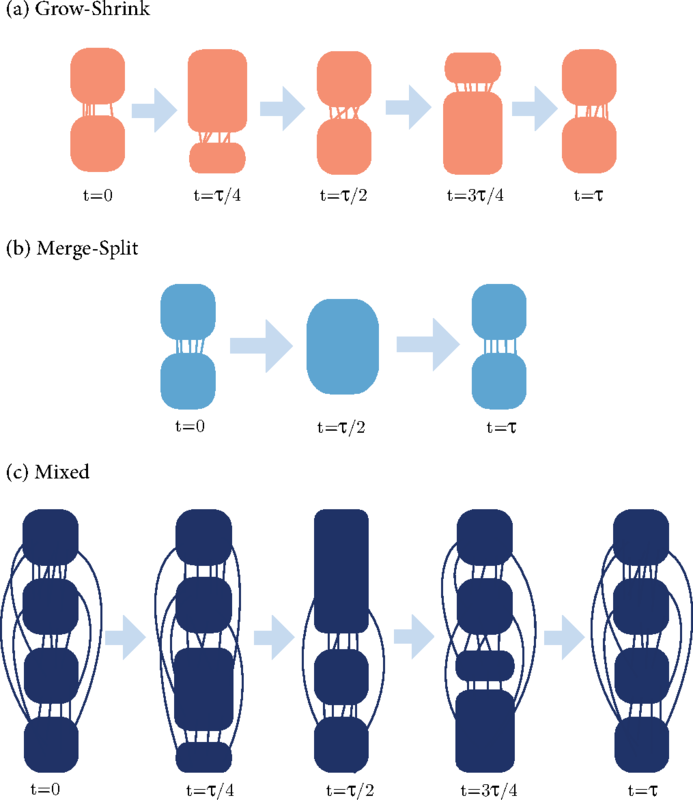
\includegraphics[width=0.3\linewidth]{img/Qualite/Granell.png}
\caption{Représentation schématique de séries de graphes pouvant générées selon différentes évolutions des communautés.\protect\footnotemark.}
\label{fig:qualite_Grannell}
\end{figure}
\footnotetext{Image provenant de \url{http://journals.aps.org/pre/abstract/10.1103/PhysRevE.92.012805}.}

Ces méthodes générent aisément des structures communautaires mais ne permettent de générer que des séries de graphes.

\subsection{Flots de liens}

Dans les flots de liens, il n'existe pas à ma connaissance de travaux étudiant la génération de flots de liens avec une structure communautaire.
Il existe principalement des méthodes étudiant les distributions de temps inter-contacts~\cite{Malmgren2008,Malmgren2009,Karsai2011,Miritello2011,Karsai2012a,Rocha2013,Vestergaard2014,Kivela2015}.
Il y a dans la littérature un large consensus sur le fait que la distribution des temps inter-contacts est souvent à queue lourde (\emph{heavy-tailed}) dans les jeux de données réel.
D'autre part, les temps inter-contacts ne semblent pas suivre un processus de Markov simple car il y a des corrélations et des effets de mémoire entre les apparitions de liens.

Toutes ces méthodes génèrent des flots de liens mais ne permettent pas de générer une structure.
Quelques méthodes se distinguent de ces travaux et génèrent une structure même si il ne s'agit pas forcément de structure communautaire.
C'est le cas des travaux de Sarnini~\emph{et al.}\cite{Starnini2013} et de Zhang~\emph{et al.}~\cite{Zhang2015a}.
Dans ces méthodes, un flot de liens est généré à partir d'un système multi-agents où chaque agent se déplace dans un espace 2D borné.
Un lien existe entre deux agents lorsqu'ils sont à distance de communication.
Dans le modèle de Zhang~\emph{et al.}, la direction prise par chaque agent n'est pas aléatoire mais en fonction de l'agent voisin étant le plus attractif.
Il s'agit donc d'un modèle de mobilité préférentielle.
Bien que ces méthodes génèrent des structures particulières dans le flot de liens, il n'existe pas de vérité de terrain sur les liens.



Barrat~\emph{et al.}~\cite{Barrat2013a} proposent une autre méthode basé sur l'utilisation de marche aléatoires.
Ils utilisent un graphe statiques pondéré et orienté qui représente l'ensemble des interactions possibles.
Ce graphe peut provenir de données réel ou être généré.
\`A partir de ce graphe, différentes marches aléatoires sont simulées sur le graphe.
Chaque marche est caractérisée par un temps de début, un n\oe uds de début, un nombre de saut et les temps séparant chaque saut.
Ces caractéristiques peuvent être définie arbitrairement ou selon des distributions données.
Chaque marche donne lieu à une liste d'interactions sous la forme $\{(t1,u0,u1), (t2,u1,u2), ..., (t_l,u_{l-1}, u_l)\}$ pour une marche de $l$ sauts.
Lors de la simulation de la marche aléatoire, le poids d'un lien dans le graphe initial est décrémenté de $1$ à chaque fois qu'il est parcouru lors d'une marche aléatoire.
Les liens du flots de liens généré sont l'union de l'ensemble des marches simulées jusqu'à ce que le graphe initial ne possède plus aucun lien.

Si le graphe statique utilisé possède une structure communautaire, il est possible que le flot de liens généré ait également une structure communautaire.
Cependant cette dépendance ne permet pas de générer des structures communautaires qui soient invisible dans le graphe statique.

\resume{
Dans le cas des séries de graphes, il existe des propositions de générateur avec structure communautaires.
Dans le cadre de flots de liens, les générateurs ne permettent pas ou alors partiellement de générer une structure donnée.
}

\section{Génération de flots de liens avec structure communautaire}
\label{sec:versqualite_methode}

Nous proposons un générateur de flots de liens sans durée s'appuyant sur une structure communautaire connue.
L'idée est de ce générateur est la suivante.
Dans un réseau de personnes, une interaction existe entre deux personnes car elle partage un point commun.
Ce point commun peut être par exemple l'intérêt pour le sport, le travail ou la famille.
Toutes les personnes partageant le même point commun interagissent entre elle de la même manière.
Cela signifie les spécificités de communications sont principalement lié à la raison de communications.
Par exemple, des collègues de travail communiquent principalement pendant la journée et rarement le soir.
Au contraire, un groupe de d'amis communiquent principalement le soir et le week end.
Avec cette hypothèse, il suffit de connaitre l'ensemble des intérêts d'une personne pour comprendre la dynamique de ses interactions.
C'est selon ce principe, proche du SBM, que nous construisons notre générateur.


L'ensemble des intérêts de l'ensemble des personnes d'un réseau se représente de la même manière que dans le SBM.
Il s'agit d'un graphe bipartie avec d'une part l'ensemble des n\oe uds et de l'autre l'ensemble des communautés.
Il existe un lien entre un n\oe ud et une communauté si le n\oe ud appartient à la communauté.
Une communauté représente un intérêt et une personne peut avoir plusieurs communautés.
Ainsi en reprenant l'exemple précédent, il existe dans le graphe bipartie autant de n\oe uds que de personnes et il y a les communautés sport, collègue et famille.

De ce graphe bipartie, les approches statiques générant un graphe déduisent la probabilité que deux n\oe uds soient reliés par un lien.
Dans le contexte de flots de liens, il ne suffit pas de calculer la probabilité qu'un lien apparaisse dans le cadre d'une communauté.
Il est nécessaire de générer un ensemble d'interactions temporelles entre ces deux n\oe uds au sein de cette communauté.
C'est pourquoi à chaque communauté est associé un processus stochastique de génération de liens qui dépend du temps.
Ainsi, chaque communauté partagée par deux n\oe ud donne lieu à la génération d'un ensemble de liens selon le processus stochastique de la communauté.
Par exemple, le processus stochastique de la communauté sport est défini par une forte activité durant les séances entrainements et une faible en dehors de ses instants.
Une représentation schématique de cette situation est présentée dans la figure~\ref{fig:qualite_Generator}.



\begin{figure}
\centering
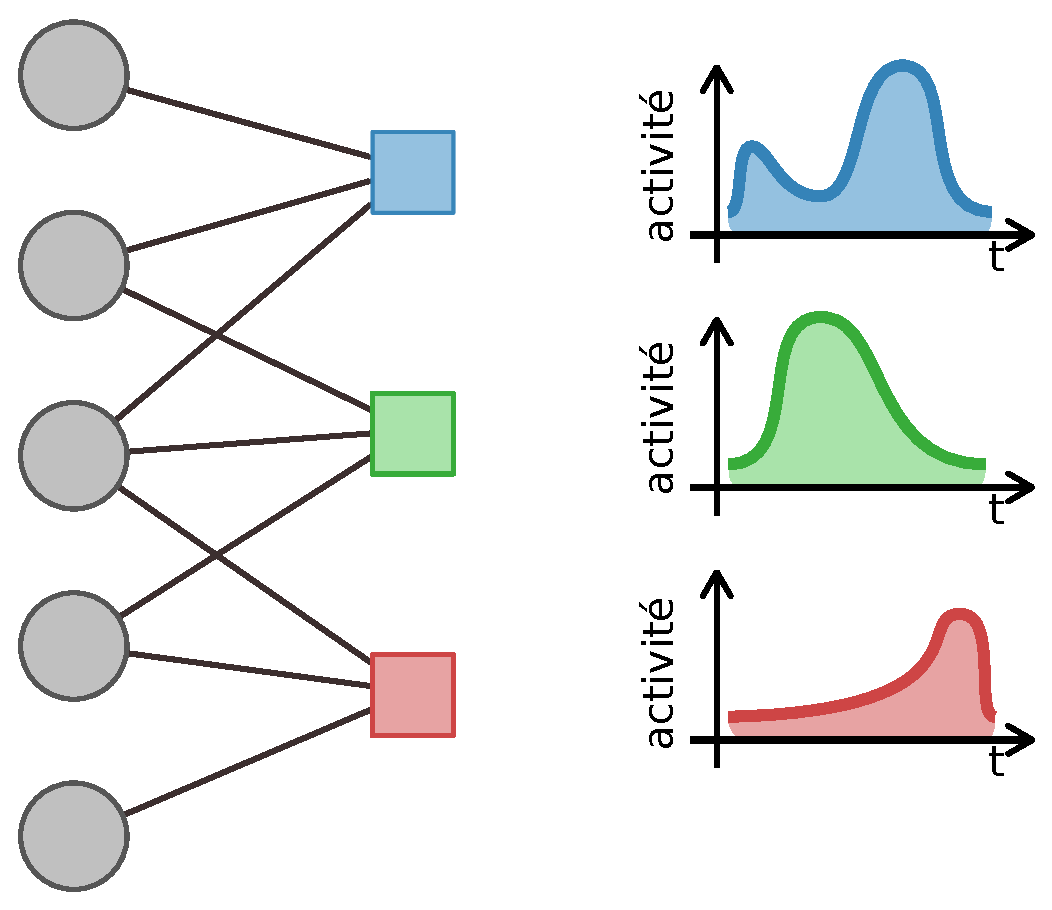
\includegraphics[width=0.5\textwidth]{img/Qualite/Generator}
\caption{Schéma de la structure communautaire considérée.
\`A gauche: un n\oe ud rond est un individu et un n\oe ud carré est une communauté.
\`A droite: Activité au cours du temps associée à chaque communauté du graphe bipartie de gauche.}
\label{fig:qualite_Generator}
\end{figure}

Le problème est alors de définir un processus de génération pour chaque communauté représentant les liens existant entre deux n\oe uds de cette communauté.
Un processus de Poisson homogène permet de générer des temps inter-contacts suivant une loi exponentielle de paramètre $\lambda$.
Cela implique que des liens apparaissent régulièrement avec une moyenne de $\dfrac{1}{\lambda}$ par unité de temps.
Or, cette hypothèse d'activité constante au cours du temps n'est pas cohérente avec notre modèle.
Si $\lambda$ varie au cours du temps, alors un processus de Poisson non-homogène est simulé et cela permet de faire varier l'activité en fonction du temps
C'est pourquoi, la distribution des temps inter-contacts des liens d'une même communauté entre deux n\oe uds est simulée via un processus de Poisson non-homogène.


Avec $N(t)$ représentant le nombre de liens existants dans l'intervalle $[\alpha,t]$, le nombre de liens entre deux instants, $a$ et $b$, suit alors la distribution suivante:
\begin{equation}
P [N(b) - N(a) = k] = \frac{e^{-\Lambda_{a,b}} (\Lambda_{a,b})^k}{k!} \qquad k= 0,1,\ldots \ ,
\end{equation}
où $\Lambda_{a,b}=\int_a^b \lambda(t)\,dt$ est l'intégrale de $\lambda$ sur $[a,b]$.
Par conséquent la probabilité qu'il y ait un et un seul lien ($k=1$) dans l'intervalle suit une loi exponentiel de paramètre $\Lambda_{a,b}$: $P [N(b) - N(a) = 1]=e^{-\Lambda_{a,b}} (\Lambda_{a,b})$.
Pour une valeur de $a$ fixée, cette probabilité est une fonction continue, croissante en fonction de $b$ et injective.
Si cette fonction également surjective si elle est strictement croissante, c'est à dire si $\Lambda_{a,b}$ est strictement croissant.

Pour générer un ensemble de liens entre une paire de n\oe uds dans une communauté, le processus est le suivant.
On commence la génération à l'instant $t_0=\alpha$ puis il est nécessaire de générer $t_1$, l'instant d'apparition du prochain lien.
Cet instant est le premier instant $t'$ tel que $N(t')- N(t_0)=1$.
La probabilité que cela arrive à cette instant est égale à $P [N(t_1) - N(t_0) = 1]=e^{-\Lambda_{t_0,t_1}} (\Lambda_{t_0,t_1})$.
Or, cette application est bijective.
Il est donc possible de l'inverser et de retrouver à partir d'une probabilité l'instant ayant cette probabilité.
Ainsi pour générer $t_1$, on génère une valeur aléatoire uniformément répartie entre $0$ et $1$.
\`A partir de cette probabilité, il suffit alors de trouver l'instant ayant exactement cette probabilité d'occurrence.
Comme $\lambda(t)$ peut être quelconque, le calcul de l'instant ayant cette probabilité se fait via une recherche dichotomique.
C'est à dire qu'un instant d'apparition de lien est choisi au hasard et sa probabilité d'occurrence est calculée, puis selon la probabilité l'instant est déplacé plus tôt ou plus tard pour se rapprocher de la probabilité voulue.
Pour générer les apparitions de liens suivantes, il suffit de recommencer ce processus à partir de $t_1$ et de chercher l'instant $t_2$ tel que $N(t_2)- N(t_1)=1$.
Un exemple de génération de temps d'apparition est présenté dans la figure~\ref{fig:qualite_Activation}.


\begin{figure}
\centering
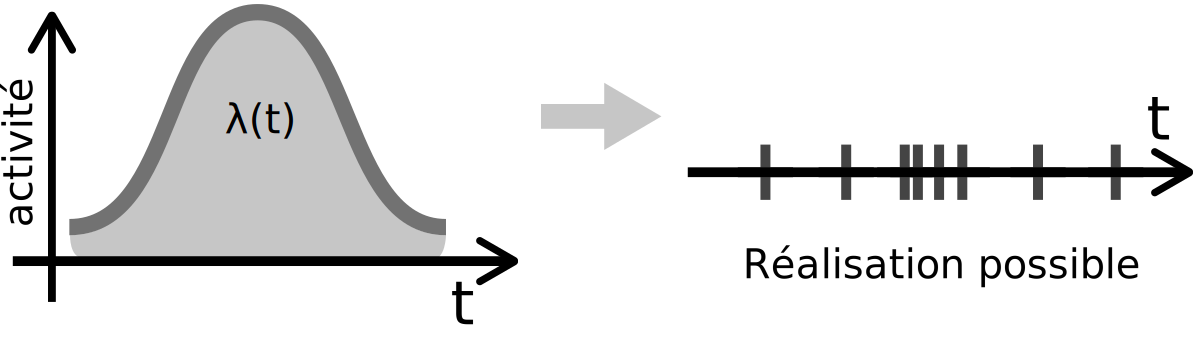
\includegraphics[width=0.7\linewidth]{img/Qualite/Activation}
\caption{Exemple des temps d'activation du lien entre deux n\oe uds donnés.}
\label{fig:qualite_Activation}
\end{figure}


En répétant le processus ci-dessus pour chaque pair de n\oe uds appartenant à une même communauté, on obtient un flot de liens avec une structure communautaire.

\subsection{Caractéristiques du générateur}

Nous discutons maintenant des situations modèlisable avec ce générateur.
Tout d'abord au seine d'une communauté, il est possible de représenter énormément d'activités temporelles différentes.
Une intensification (resp. baisse) des interactions au cours du temps est représentée par une activité croissante (resp. décroissante).
Il est possible représenter des réunions cycliques par une activité cyclique avec une activité positive uniquement lors des réunions. 
Ce modèle d'activations des liens reste  cependant une approximation car il n'y a aucune prise en compte des possibles corrélations au sein d'une communauté.
De même, l'ensemble des paires de n\oe uds d'une communauté sont des processus indépendant et identiquement distribué.
Il n'y a donc au sein d'une communauté aucune différence entre les n\oe uds.
Il n'est, de plus, pas possible de représenter l'intégration progressive d'un n\oe ud à une communauté.

Vis-à-vis de l'ensemble des communautés, le modèle est encore une fois assez libre car un n\oe ud peut appartenir à plusieurs communautés.
Chaque communauté est traitée de manière indépendante et une même paire de n\oe uds peut donner lieu à la génération de liens de différentes communautés selon plusieurs processus indépendants.
Ainsi même si les n\oe uds sont équivalent au sein d'une communauté, il existe tout de même une hétérogénéité des n\oe uds en fonction du nombre de communautés auquel il appartient.

\bigskip

Avec cette formulation, le générateur dépend du graphe bipartie d'affiliation des n\oe uds aux communautés et de l'activité temporelle de chaque activité.
L'approche que suivons est purement générative.
Le but n'est donc pas d'inférer ces paramètres sur un exemple mais de pouvoir les fixer manuellement.
Afin de faciliter l'utilisation de ce générateur, nous utilisons différentes méthodes pour fixer ces nombreux paramètres dans la section suivante.


\section{Applications}
\label{sec:versqualite_Applications}

Il est donc possible de créer des flots de liens ayant une vérité de terrain sur les liens.
Les paramètres générant le flot de liens et la vérité de terrain associé peuvent être minutieusement choisis afin que le flot de liens exhibe des caractéristiques spécifiques.
C'est cette approche que nous utilisons pour tester deux méthodes de détection statique dans la sous-section~\ref{sec:versqualite_statique}.

Les paramètre peuvent être choisi aléatoirement selon certain critère  afin de générer des structures plus diverses.
C'est cette approche que nous utilisons pour l'étude de fonctions de qualité dans la sous-section~\ref{sec:versqualite_qualite}.



\subsection{Étude de méthodes statiques}
\label{sec:versqualite_statique}

Lors de la génération de graphes statiques avec structure communautaire chevauchante, il y a principalement deux critères impactant une réalisation: la densité à l'intérieur d'une communauté et le chevauchement de la structure.
Dans le cas des flots de liens, il faut aussi ajouter le chevauchement temporelle.
C'est pourquoi, nous générons différentes situations avec recouvrement topologique et/ou temporelle des communautés. 
Ces types de génération sont présentés dans la figure~\ref{fig:versqualite_gen_test}.
Il s'agit d'un exemple avec $15$ n\oe uds pendant $30$ unité de temps où il existe cinq communautés qui dure chacune $10$ unité de temps.
Afin de simplifier la méthode de tests, chaque communauté a une activité constante durant l'intervalle où elle existe.
Avec ces paramètre fixés, nous étudions quatre type de flots de liens qui sont représentés dans les figures suivantes:

\begin{description}
\item[\ref{fig:versqualite_gen_test1}] chaque communauté est bien séparée des quatre autres. Il s'agit de l'exemple le plus simple car il n'y a aucun chevauchement topologique des communautés;
\item[\ref{fig:versqualite_gen_test2}] il n'y aucun chevauchement temporel mais il existe un chevauchement topologique au niveau de la communauté trois;
\item[\ref{fig:versqualite_gen_test3}] il y a un léger chevauchement topologique entre les communautés $1$ et $2$ et entre les communautés $4$ et $5$.
\item[\ref{fig:versqualite_gen_test4}] il y a un fort chevauchement topologique entre les communautés $1$ et $2$ et entre les communautés $4$ et $5$.
\end{description}


 
\begin{figure}
\centering
	\begin{subfigure}{0.3\textwidth}
		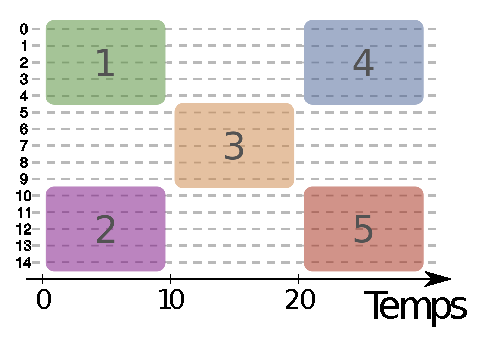
\includegraphics[width=\textwidth]{img/Qualite/topologie1.eps}
		\caption{}
		\label{fig:versqualite_gen_test1}
	\end{subfigure}\hspace*{0.1\textwidth}
	\begin{subfigure}{0.3\textwidth}
		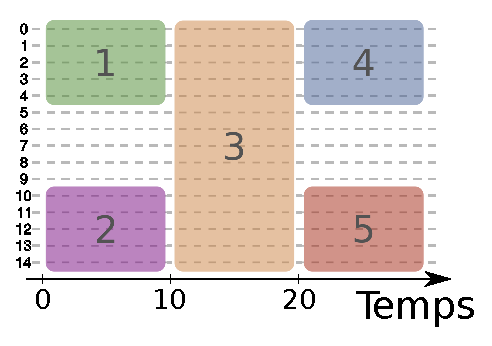
\includegraphics[width=\textwidth]{img/Qualite/topologie2.eps}
		\caption{}
		\label{fig:versqualite_gen_test2}
	\end{subfigure}
	
	\begin{subfigure}{0.3\textwidth}
		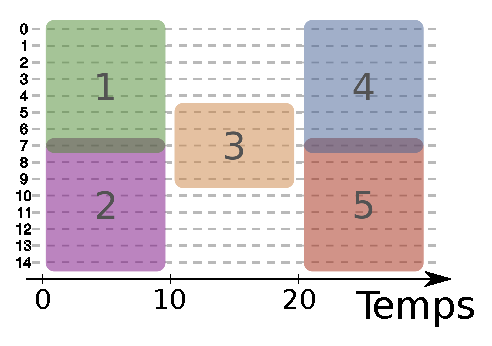
\includegraphics[width=\textwidth]{img/Qualite/topologie3.eps}
		\caption{}
		\label{fig:versqualite_gen_test3}
	\end{subfigure}\hspace*{0.1\textwidth}
	\begin{subfigure}{0.3\textwidth}Une
		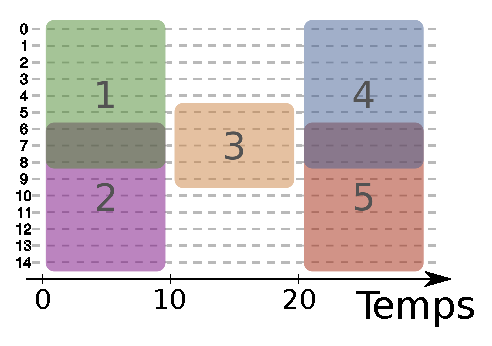
\includegraphics[width=\textwidth]{img/Qualite/topologie4.eps}
		\caption{}
		\label{fig:versqualite_gen_test4}
	\end{subfigure}	
	\caption{Représentation schématique de quatre types de flot de liens ayant une structure communautaire avec 5 communautés.
	Chaque rectangle de couleur représente une communauté ayant une activité constante.}
	\label{fig:versqualite_gen_test}
\end{figure}

\bigskip
Pour chacun de ses type de flots de liens, nous avons appliqué une méthode d'optimisation de modularité~\cite{Blondel2008a} et une méthode de communauté égo-centrée~\cite{Danisch2012} sur une projection du flot de liens en un graphe statique.
Ces méthodes ont été présentées dans le chapitre~\ref{chap:etat_art}.


Nous avons défini  dans le chapitre une projection du flot de liens en un graphe statique dans le cas où les liens ont une durée.
Dans les flots de liens générés, il n'y a pas de durée sur les liens.
C'est pourquoi nous utilisons une projection différentes qui transforme le flot de liens en un graphe statique pondéré.
Chaque lien du flot est toujours représenté par un n\oe ud dans le graphe statique et il y un lien entre deux n\oe uds du graphe statique si les liens correspondants ont un n\oe uds en commun.
Afin de tenir compte de la séparation temporelle, un lien dans le graphe statique est pondéré par une fonction décroissante dépendante du temps séparant les deux liens dans le flot.
Nous avons choisi comme fonction décroissante: $e^{-\lambda d}$ où $d$ est le temps séparant les deux liens et $\lambda$ une constante positive.
Ainsi, les poids de la projection sont répartis entre $0$ et $1$.
Dans la suite, nous avons à chaque fois fait varier $\lambda$ de manière exhaustive.
Plus $\lambda$ a une valeur importante, plus le temps a de l'importance.
Par exemple pour $\lambda=3$, une séparation temporelle de $1$ unité de temps donne lieu à poids de $0.05$ dans la projection.
Dans cette situation, le graphe de la projection ne capture plus vraiment de relation topologique car un lien n'est alors relié que avec ses voisins les plus proches.
Dans le cas inverse quand $\lambda$ est égale à zéro, la projection du flot de liens est complètement identique au \emph{line-graph} du multigraphe agrégé.

Lors de nos tests,  nous avons comparé visuellement\,\footnote{Une évaluation plus quantitative avec la \emph{NMI} est possible mais ne semble pas nécessaire à cette étape.} la vérité de terrain et la meilleure partition trouvée par la méthode de Louvain et la méthode proximité CarOp selon le $\lambda$ choisi.
La méthode CarOp nécessite d'initialiser les communautés avec un lien.
Nous choisissons pour chaque  communauté un lien apparaissant au milieu de sa duré de vie; par exemple un lien à l'instant $15$ est choisi pour initialiser une communauté qui sera \emph{a prioi} proche de la communauté $3$.

Dans ce cadre, nous observons que les deux méthodes sont capables de retrouver la structure exhibée dans la figure~\ref{fig:versqualite_gen_test1}.

La structure présentée dans la figure~\ref{fig:versqualite_gen_test2} est retrouvée par CarOp mais non par Louvain.
La communauté $3$ n'est jamais détectée par Louvain peu importe le $\lambda$ utilisé pour la projection.
Selon la valeur de $\lambda$, les liens de la communauté $3$ sont soit répartis entre les autres communautés soit répartis en plusieurs communautés autonomes.
En effet, cette méthode utilise la modularité sur une structure proche du \emph{line-graphe} d'un multigraphe.
Elle est donc proche des méthodes de Evans~\emph{et al.}~\cite{Evans2009} que nous avons présentés dans la section~\ref{sec:expected_travaux} et souffre des même biais\,\footnote{Plus une clique d'un graphe est grande, moins sa transformation dans le \emph{line-graph} est dense.}.

La structure présentée dans la figure~\ref{fig:versqualite_gen_test3} est retrouvée par Louvain mais non par CarOp.
Comme les communautés de liens sont plus petites et ne se chevauchent que peu, la méthode de Louvain arrive à capturer les différentes partitions.
La méthode CarOp, quant à elle, n'est pas capable de différencier les communautés $1$ et $2$.
CarOp détecte comme communauté des ensembles de n\oe uds proche dans la projection.
Or, un lien au début de la communauté $1$ est plus proches des liens au débuts de la communauté $2$ que des liens à la fin de la communauté $1$.
C'est pourquoi, CarOp ne différencie pas les communautés $1$ et $2$.

La structure présentée dans la figure~\ref{fig:versqualite_gen_test4} n'est retrouvée ni par la de Louvain ni par CarOp.
Comme la situation dans la figure~\ref{fig:versqualite_gen_test4} est proche de celle dans la figure~\ref{fig:versqualite_gen_test3}, il est normal que CarOp ne parvienne toujours pas à différencier les communautés $1$ et $2$.
Pour la méthode de Louvain, les communautés $1$ et $2$ ne sont pas détectées.
Pour des valeurs faible de $\lambda$, les communautés $1$ et $2$ sont séparés en  $4$ ou $5$ plusieurs communautés sans logique apparentes.
Pour des valeurs élevés de $\lambda$, il existe bien deux communautés correspondants aux communautés $1$ et $2$ mais la partie chevauchante est complètement intégrée dans l'une de ces deux communautés.



\resume{
Il s'agit de premier tests sur des méthodes existantes de détections statique de communautés sur la projection du flot de liens en un graphe pondéré.
Les méthodes que nous avons testés ne permettent pas de capturer l'ensemble des topologiques généré par notre générateur.
Ce fait est attendu car nous les appliquons sur des projections du flots de liens.
Il est toute fois intéressant qu'il est possible de retrouver la vérité de terrain par une méthode statique dans certaines conditions.
}

\subsection{Étude de fonctions de qualité}
\label{sec:versqualite_qualite}

\section{Conclusion}


\subsection{Perspectives}

test plus quantitaifs sur les méthodes existantes et sur l'impacte de l'activité.

étude de la vraisemblence des flots de liens généré et l'inférence de quelques paramètres.

Ajout de durée selon une distribution

Preferential attachment temporel

